\documentclass[tikz,border=10pt]{standalone}
\usepackage{tikz}
\usetikzlibrary{positioning,shapes.geometric}

\begin{document}
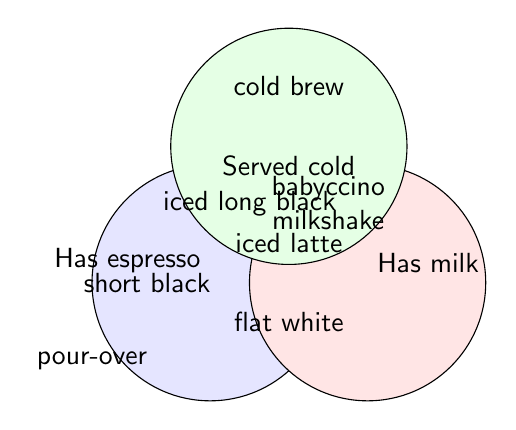
\begin{tikzpicture}[font=\sffamily]
    % Define circle centers
    \coordinate (A) at (0,0); % Has espresso
    \coordinate (B) at (2,0); % Has milk
    \coordinate (C) at (1,1.732); % Served cold

    % Draw circles
    \draw[fill=blue!10] (A) circle (1.5cm) node[above left] {Has espresso};
    \draw[fill=red!10] (B) circle (1.5cm) node[above right] {Has milk};
    \draw[fill=green!10] (C) circle (1.5cm) node[below] {Served cold};

    % Place drinks in regions
    % Short black: only espresso
    \node at (-0.8,0) {short black};

    % Flat white: espresso + milk (bottom intersection)
    \node at (1,-0.5) {flat white};

    % Iced latte: all three
    \node at (1,0.5) {iced latte};

    % Iced long black: espresso + cold (left top)
    \node at (0.5,1.0) {iced long black};

    % Cold brew: only cold (top)
    \node at (1,2.5) {cold brew};

    % Babyccino: milk + cold (right top)
    \node at (1.5,1.2) {babyccino};

    % Milkshake: milk + cold (right top)
    \node at (1.5,0.8) {milkshake};

    % Pour-over: none
    \node at (-1.5,-1) {pour-over};

\end{tikzpicture}
\end{document}
